\section{Arquitectura}
\label{sec:arquitectura}

A continuación se presentan los detalles de implementación del sistema propuesto. La solución propuesta está basada en FCD obtenido mediante dispositivos móviles. La información obtenida es procesada en el servidor utilizando un algoritmo de MM y el resultado es almacenado en una base de datos GIS para consultas a través de una aplicación móvil y una página web desarrolladas para el efecto.

En la \Cref{fig:arquitectura} se ilustra la arquitectura modular del sistema desarrollado. La plataforma cuenta con tres componentes principales:
\begin{enumerate*}[1)] \item una base de datos GIS que almacena el mapa de calles y las trayectorias de muestra de los vehículos, \item una aplicación móvil que captura los datos del trayecto recorrido por los vehículos y \item una aplicación web que procesa los datos obtenidos y genera información sobre el estado del tránsito.  
\end{enumerate*}

\begin{figure}[h*]
	\centering
	\input{apartados/figuras/arquitectura.pdf_tex}
	\caption{\label{fig:arquitectura} Arquitectura del Sistema}	
\end{figure}

\subsection{Almacenamiento de datos}
\label{base-de-datos}

A modo de generar información sobre el estado del tráfico de un área geográfica en particular, se debe contar con un mapa de calles y con un conjunto de trayectorias obtenidas mediante FCD durante un período de tiempo determinado.

El mapa de calles es obtenido de Open Street Maps\footnote{http://www.openstreetmap.org/} (OSM) y almacenado en una base de datos GIS como un grafo dirigido, donde los vértices corresponden a las intersecciones de las calles y las aristas corresponden a los segmentos de calles. La longitud de cada calle determina su peso, que es utilizado para el cálculo del camino más corto.

Por otro lado, para almacenar la información de las trayectorias de muestra de los usuarios se definen las siguientes tablas en la base de datos GIS:
\begin{enumerate}
\item \textbf{Localizaciones}: En esta tabla se guardan los datos de ubicación que son recibidos periódicamente de los usuarios de la aplicación móvil. Se almacena la fecha, la latitud, la longitud, la velocidad, la dirección, la precisión, altitud y la trayectoria a la que pertenece.
\item \textbf{Rutas}: Una ruta es un conjunto de localizaciones que sirven como dato de entrada para el proceso de MM. Cada ruta representa una muestra de una trayectoria recorrida por el usuario durante un viaje.
\end{enumerate}

\subsection{Implementación de FCD}
\label{floating-car-data}

La información de FCD es obtenida por medio de una aplicación móvil desarrollada como parte del presente trabajo que ha sido denominada Autotracks\footnote{https://play.google.com/store/apps/details?id=py.com.fpuna.autotracks}. La misma se encarga de capturar, almacenar y enviar periódicamente a un servidor central las muestras de las trayectorias de los usuarios que están en un vehículo en movimiento. Para este propósito, Autotracks cuenta con tres componentes principales: 

\subsubsection{Reconocimiento de actividad}
\label{reconocimiento_actividad}

El reconocimiento de actividad consiste en determinar la acción que está realizando una persona en base a un patrón de movimientos observados mediante los sensores con los que cuentan los dispositivos móviles, como el acelerómetro, el giroscopio y los dispositivos GPS integrados. En Autotracks se utiliza una implementación proveída como parte de \emph{Google Play Services}\footnote{http://developer.android.com/google/play-services/index.html}, denominada \emph{Activity Recognition}\footnote{http://developer.android.com/training/location/activity-recognition.html} para determinar cuando un usuario se encuentra en un vehículo en movimiento.

El \Cref{alg:deteccion_actividad} muestra el procedimiento ejecutado periódicamente cada vez que se obtiene un resultado del reconocimiento de actividad. Este procedimiento verifica si la toma de localizaciones está o no iniciada y se encarga de iniciarla o finalizarla de acuerdo a la actividad detectada. El resultado de la detección es almacenado para ser utilizado en la siguiente invocación del procedimiento. Si se ha detectado movimiento, el tiempo en el que ocurrió la detección también es almacenado.
 
\begin{algorithm}
\caption{Reconocimiento de Actividad}
\label{alg:deteccion_actividad}
\begin{algorithmic}[1]
\Procedure{ActividadDetectada}{$actividad$}
	\State $enVehiculo =$ \Call {EstaEnVehiculo}{$actividad$}
%	\State Guardar $enVehiculo$ como el último estado detectado  
	\If {$enVehiculo$}
		\State $ultimoEstado = \text{VEHICULO}$
		\If {RASTREO no está iniciado}
			\State Iniciar RASTREO
		\EndIf
	\Else
		\State $ultimoEstado = null$
		\If {RASTREO está iniciado}
			\State Finalizar RASTREO
		\EndIf
	\EndIf
\EndProcedure
\Statex
\Function {EstaEnVehiculo}{$actividad$}
	\If {$actividad == \text{A\_PIE}$}
		\State \Return $falso$
	\Else
		\State Inicializar $t$ al tiempo actual
		\If {$actividad == \text{VEHICULO}$}
			\State $t\_ultimaDeteccion = t$ 
			\State \Return $verdadero$
		\Else
		\If {$ultimoEstado == \text{VEHICULO}$}
			\State $\Delta t = t - t\_ultimaDeteccion$
			\If {$\Delta t \leq$ TOLERANCIA}
				\State \Return $verdadero$
			\Else
				\State \Return $falso$
			\EndIf
		\Else
			\State \Return $falso$
		\EndIf
		\EndIf
	\EndIf
\EndFunction
\end{algorithmic}
\end{algorithm}

\subsubsection{Toma de localizaciones}
\label{toma_localizaciones}

La ubicación de los teléfonos móviles puede ser obtenida utilizando triangulación de antenas de telefonía, puntos de acceso WiFi con ubicaciones conocidas o mediante el uso de los satélites GPS. A fin de tener la mayor flexibilidad posible, Autotracks es capaz de trabajar con cualquiera de estas opciones, para ello se utiliza una implementación denominada \emph{Fused Location Provider}\footnote{http://developer.android.com/training/location/receive-location-updates.html}.

En los casos en los que la localización es obtenida a través de las redes GSM o WiFi no se dispone de la información de velocidad, la cual es necesaria para el procesamiento posterior. Para paliar esta falta de información, la velocidad es estimada utilizando la localización anterior, si la misma está disponible, de la siguiente manera: \begin{equation} \label{eq:velocidad} v=\frac { d }{ t } \end{equation} donde $d$ es la distancia entre la localización actual y la anterior, y $t$ es el tiempo que transcurrió entre la toma de las localizaciones.

Para evitar registrar localizaciones erróneas se utilizan dos métodos de filtrado. El primer método consiste en descartar las localizaciones que reportan un error de precisión mayor a un máximo preestablecido. El segundo método consiste en determinar la velocidad de viaje entre dos puntos consecutivos utilizando la \cref{eq:velocidad}, si es mayor a un valor preestablecido la localización es descartada. Además, también se descartan las localizaciones que son muy próximas entre sí. En el \Cref{alg:toma_de_localizaciones} se describe el procedimiento utilizado para registrar una localización.

\begin{algorithm}
\caption{Toma de Localizaciones}
\label{alg:toma_de_localizaciones}
\begin{algorithmic}[1]
\Procedure {Registrar}{$localizacion$}
	\State $esValida = \Call{EsValida}{localizacion}$
	\If {$esValida$}
		\State $ultimaLocalizacion = localizacion$
	\EndIf
\EndProcedure
\Statex
\Function {EsValida}{$localizacion$}
	\State Inicializar $p$ a la precisión de la $localizacion$	
	\State $\Delta d = \Call{Distancia}{localizacion, ultimaLocalizacion}$
	\State $\Delta t = \Call{Tiempo}{localizacion, ultimaLocalizacion}$
	\State $v = \Delta d / \Delta t$
	\If {$\Delta d > \text{D\_MIN} \land v < \text{V\_MAX} \land p < \text{P\_MAX}$}
	    \State \Return $verdadero$
	\Else
	    \State \Return $falso$
	\EndIf
\EndFunction
\end{algorithmic}
\end{algorithm}

\subsubsection{Envío de datos}

La aplicación envía los datos de las localizaciones a través de Internet a un servidor central que se encarga de almacenar y procesar la información. Para disminuir el consumo de batería ocasionado por la utilización de la red de datos móviles, los teléfonos almacenan temporalmente las localizaciones capturadas y las envían periódicamente al servidor.

Para enviar las localizaciones no es necesario que el usuario haya finalizado completamente su recorrido, todas las localizaciones capturadas durante un periodo de tiempo definido son enviadas al servidor. El resto de las localizaciones del mismo recorrido son enviadas en los siguientes periodos. De esta forma los recorridos parciales pueden ser utilizados para estimar el estado del tráfico aproximadamente en tiempo real.

\subsection{Implementación de MM}
\label{implementacion_mm}

Un proceso de Map Matching (MM) es ejecutado cada vez que las muestras de las trayectorias de los vehículos son enviadas desde los teléfonos móviles al servidor central para determinar el camino real recorrido por cada vehículo. En este proceso se utiliza el algoritmo conocido como ST-Matching\cite{lou2009map} con las mejoras propuestas por \cite{budigm2012algorithm} y \cite{sakic2012map}. 

ST-Matching es un algoritmo topológico específicamente diseñado para funcionar de forma \emph{off-line} y con intervalos de tiempo relativamente largos entre las muestras. Estas características se adecuan a los requerimientos impuestos por la arquitectura de la solución propuesta.  El algoritmo consta de tres partes principales: \begin{enumerate*}[a)]
\item la \emph{Selección de Candidatos},
\item el \emph{Análisis Espacial y Temporal} y
\item la \emph{Obtención del Resultado}.
\end{enumerate*}

Los datos de entrada del algoritmo de MM son la red de calles, que se describió en el \cref{base-de-datos}, y la muestra de la trayectoria de un vehículo, obtenida mediante el uso de la aplicación móvil, como se explica en el \cref{floating-car-data}. El resultado de este procesamiento es una aproximación del camino real recorrido por el vehículo.

La red de calles es modelada como un grafo dirigido $G(V,E)$, donde $V$ es el conjunto de todos los vértices correspondientes a las intersecciones y extremos de los segmentos de calles, y $E$ es el conjunto de todas las aristas que representan segmentos de calles. Además, cada segmento $e \in E$ tiene como datos un identificador único $e.id$, el límite de velocidad $e.v$ de la calle, la longitud $e.l$ del segmento, el identificador del vértice inicial $e.ini$ y el del vértice final $e.fin$. En la \Cref{fig:segmentos_de_calle} se aprecia como una calle puede estar dividida en varios segmentos, donde cada segmento está comprendido entre dos vértices del mapa.

\begin{figure}[h*]
	\centering
	\input{apartados/figuras/segmentos_calle.pdf_tex}
	\caption{\label{fig:segmentos_de_calle} Representación de segmentos de calles}	
\end{figure}

La trayectoria de muestra $T$ de un vehículo es representada como una secuencia ordenada de puntos $p_1, p_2, \dots, p_n$ donde cada punto $p_i$ tiene además como datos su latitud $p.lat$, su longitud $p.lon$, su velocidad aproximada $p.v$, su dirección de desplazamiento $p.d$ y el tiempo $p.t$ en que fue tomada la muestra. Esta trayectoria está ordenada con respecto al tiempo de tal manera que $p_i.t < p_{i + 1}.t$ para $1 \le i < n$. La \Cref{fig:trayectoria} muestra un ejemplo de una trayectoria correspondiente a un vehículo de prueba.

\begin{figure}[h*]
	\centering
	\input{apartados/figuras/trayectoria_vehiculo.pdf_tex}
	\caption{\label{fig:trayectoria} Trayectoria de un vehículo}	
\end{figure}

El camino real $R$ es definido como una secuencia de segmentos de calles $e_i$ conectados entre sí, que se inicia en un vértice $v_{ini} \in V$ y finaliza en un vértice $v_{fin} \in V$, es decir, $R = \{ e_1, e_2, \dots, e_n \}$, donde $e_1.ini = v_{ini}$, $e_n.fin = v_{fin}$ y $e_i.fin = e_{i + 1}.ini$ para $1 \le i < n$.

\subsubsection{Selección de Candidatos}
\label{seleccion_de_candidatos}

La primera etapa del proceso es la selección de puntos candidatos. Un punto candidato $c$ es un punto perteneciente a un segmento de calle $e$, que puede formar parte del camino real recorrido por un vehículo, y que es obtenido a partir de un punto $p$ de una trayectoria de muestra. Dada una trayectoria de muestra $T = \{p_1, p_2, \dots, p_n\}$, el proceso de selección de candidatos consiste en encontrar para cada punto $p_i$, $1\le i\le n$, el conjunto de puntos candidatos $C_i = \{c_{i}^{1}, c_{i}^{2}, \dots, c_{i}^{m}\}$ correspondiente.

El primer paso es seleccionar todos los segmentos de calles $e \in E$ tales que la distancia entre un punto $p_i$ y un segmento $e$ sea menor a un radio $r$, de esta forma se obtiene un conjunto de segmentos $E_i = \{ e : \text{ } e \in E \text{ } \wedge \text{ } dist(p_i, e) < r \}$. Luego, para cada segmento $e_{i}^{j}$ perteneciente al conjunto $E_i = \{e_{i}^{1}, e_{i}^{2}, \dots, e_{i}^{m}\}$ resultante, se obtiene un punto candidato $c_{i}^{j}$ realizando una proyección del punto $p_i$ sobre el segmento $e_{i}^{j}$. La proyección $proy(p, e)$ de un punto $p$ sobre un segmento $e$ se define como el punto $c$ perteneciente a $e$ más cercano a $p$, es decir, $c = \text{arg } min(dist(c_i, p)) \text{ } \forall c_i \in e$. Así, se obtiene el conjunto de puntos candidatos $C_i = \{ proy(p_i, e_j) \text{ } \forall e_j \in E_i \}$. Como se puede apreciar en la \Cref{fig:puntos_candidatos} un punto candidato puede ser cualquier punto del segmento, como en el caso de $c_{i}^{1}$ y $c_{i}^{2}$, o uno de sus vértices como en el caso de $c_{i}^{3}$.

\begin{figure}[h*]
	\centering
	\input{apartados/figuras/puntos_candidatos.pdf_tex}
	\caption{\label{fig:puntos_candidatos} Puntos candidatos para un punto de la trayectoria}	
\end{figure}

Una vez que se han obtenidos todos los conjuntos $C_i = \{c_{i}^{1}, c_{i}^{2}, \dots, c_{i}^{m}\}$ correspondientes a cada punto $p_i$ de la trayectoria de muestra $T$, el problema de MM se reduce a cómo seleccionar un punto candidato $c_i$ de cada conjunto $C_i$, a partir del cual se obtiene el segmento de calle $e_i$, de manera tal que el camino real resultante $R = \{ e_1, e_2, \dots, e_n \}$ sea lo más aproximado posible a $T = \{ p_1, p_2, \dots, p_n\}$.

\subsubsection{Análisis Espacial y Temporal}

La segunda etapa del proceso tiene por objetivo seleccionar el punto candidato $c_i$ de cada conjunto $C_i$ que sea el más apropiado para cada punto $p_i$ de la trayectoria de muestra. Para ello cada punto candidato y cada posible conexión entre dos puntos candidatos consecutivos son analizados de acuerdo a dos criterios de calidad, el \emph{análisis espacial} y el \emph{análisis temporal}.

En el análisis espacial se utiliza información geométrica y topológica de la red de calles para evaluar los puntos candidatos. La información geométrica es incorporada utilizando la \emph{probabilidad de observación} y la información topológica es expresada utilizando la \emph{probabilidad de transmisión}.

La \emph{probabilidad de observación} es la probabilidad de que un punto candidato $c_{i}^{j}$ corresponda a un punto $p_i$ de la trayectoria de muestra, calculada en base a la distancia $dist(c_{i}^{j},p_i)$ entre los puntos. Asumiendo que el error en la medición de la posición de $p_i$ sigue una distribución normal, la probabilidad de observación $N(c_{i}^{j})$ se define como
\begin{equation} \label{probabilidad_de_observacion}
N(c_{i}^{j}) = \frac {1}{\sqrt { 2 \pi \sigma }} {e}^{\frac {{(x_{i}^{j} - \mu)}^{2}}{{ 2 \sigma}^{2}}}
\end{equation}
donde $x_{i}^{j} = dist(c_{i}^{j},p_i)$ es la distancia entre $p_i$ y el punto candidato $c_{i}^{j}$. 
La \emph{probabilidad de transmisión} se define como la probabilidad de que el camino más corto entre un punto candidato $c_{i-1}^{j}$ y el siguiente punto candidato $c_{i}^{k}$ es el camino correcto de $p_{i-1}$ a $p_i$. La probabilidad de transmisión se calcula de la siguiente forma: 
\begin{equation} \label{probabilidad_de_transmision}
V(c_{i-1}^{j}, c_{i}^{k}) = \frac { min( dist(p_{i-1}, p_i), long(c_{i-1}^{j}, c_{i}^{k})) }{ max (dist(p_{i-1}, p_i), long(c_{i-1}^{j}, c_{i}^{k})) }
\end{equation}
donde $long(c_{i-1}^{j}, c_{i}^{k})$ es la longitud del camino más corto entre $c_{i-1}^{j}$ y $c_{i}^{k}$. El cálculo del camino más corto se realiza utilizando el algoritmo de Dijkstra\footnote{http://es.wikipedia.org/wiki/Algoritmo\_de\_Dijkstra} para grafos dirigidos. La dirección de las aristas del grafo representan el sentido de circulación de la calle, de esta forma se incorpora información topológica en el análisis espacial.

Combinando la \Cref{probabilidad_de_observacion} y la \Cref{probabilidad_de_transmision} se define la función de análisis espacial $F_s(c_{i-1}^{j},c_{i}^{k})$ como el producto de la probabilidad de observación y la probabilidad de transmisión de la siguiente forma:
\begin{equation} \label{funcion_espacial}
F_s(c_{i-1}^{j},c_{i}^{k}) = N(c_{i}^{k}) \times V(c_{i-1}^{j}, c_{i}^{k}), \quad 2 \le i \le n 
\end{equation}

Como resultado del análisis espacial se asigna un valor numérico a todos los posibles caminos que van de $p_{i-1}$ a $p_i$ obtenido mediante la \Cref{funcion_espacial}.

En el análisis temporal se calcula la velocidad promedio entre dos puntos consecutivos $p_{i-1}$ y $p_i$ y se compara con los límites de velocidad de los segmentos de calles comprendidos entre dos puntos candidatos $c_{i-1}^{j}$ y $c_{i}^{k}$ con el fin de seleccionar el segmento cuya velocidad promedio es la más cercana a la velocidad promedio de desplazamiento del vehículo.

Dados dos puntos candidatos $c_{i-1}^{j}$ y $c_{i}^{k}$ correspondientes a dos puntos consecutivos $p_{i-1}$ y $p_i$ respectivamente, el camino más corto entre $c_{i-1}^{j}$ y $c_{i}^{k}$ es una lista de segmentos $[e_1, e_2, \dots, e_n]$. La velocidad promedio de desplazamiento del vehículo en ese camino más corto se define como:
\begin{equation}
\overline{v} = \frac { \sum_{m=1}^{n} {e_m.l} }{ \Delta t_{i-1, i} }
\end{equation}
donde $e_m.l$ es la longitud del segmento $e_m$ y $\Delta t_{i-1, i} = p_i.t - p_{i-1}.t$ es el intervalo de tiempo entro dos puntos consecutivos de la trayectoria de muestra. Además, cada segmento $e_m$ tiene una velocidad $e_m.v$ correspondiente al límite de velocidad de la calle. La Similaridad Coseno\footnote{http://es.wikipedia.org/wiki/Similitud\_coseno} es utilizada para medir la semejanza entre $\overline{v}$ y los límites de velocidad. De esta forma, la función de análisis temporal queda definida así:
\begin{equation} \label{funcion_temporal}
F_{ t }(c_{ i-1 }^{ j },c_{ i }^{ k })=\frac { \sum _{ m=1 }^{ n }{ (e_{ m }.v\times \overline { v } ) }  }{ \sqrt { \sum _{ m=1 }^{ n }{ (e_{ m }.v)^{ 2 } }  } \times \sqrt { \sum _{ m=1 }^{ n }{ (\overline { v } )^{ 2 } }  }  } 
\end{equation}

\subsubsection{Búsqueda del Resultado}

\label{busqueda_de_resultado}
El resultado de los procesos descritos anteriormente es un grafo acíclico dirigido de puntos candidatos, que representa todos los posibles caminos entre el punto inicial $p_1$ y el punto final $p_n$ de la trayectoria de muestra $T$. Como se muestra en la \Cref{fig:grafo_de_candidatos}, los nodos del grafo corresponden a los candidatos de cada punto $p_i$ y las aristas representan los caminos más cortos entre cada par de candidatos $c_{i-1}^j$ y $c_i^k$ consecutivos. A cada arista se le asigna un peso de acuerdo a la probabilidad de transmisión entre su vértice inicial y final, y a la probabilidad de observación del vértice inicial.

\begin{figure}[h*]
	\centering
	\input{apartados/figuras/grafo_puntos_candidatos.pdf_tex}
	\caption{\label{fig:grafo_de_candidatos} Grafo de puntos candidatos}	
\end{figure}

Para asignar el peso a cada arista se combinan la \cref{funcion_espacial} y la \cref{funcion_temporal} definiendo así la función espacio-temporal de la siguiente forma:
\begin{equation} \label{funcion_espacio_temporal}
F(c_{i-1}^{j},c_{i}^{k}) = F_s(c_{i-1}^{j},c_{i}^{k}) \times F_{ t }(c_{ i-1 }^{ j },c_{ i }^{ k }), 2 \leq i \leq n
\end{equation}

Dada una secuencia de puntos candidatos $C_T = \{c_1, c_2, \dots, c_n\}$, el peso global se define como $F(C_T) = \sum _{ i=2 }^{ n }{F(c_{i-1}^{j},c_{i}^{k})}$, es decir, es la sumatoria de los pesos de todas las aristas que componen la secuencia. El objetivo del algoritmo es obtener la secuencia que tenga el mayor peso.

El \Cref{alg:st_matching} muestra los pasos realizados para obtener la secuencia de puntos candidatos. El primer paso es construir el grafo $G_T$ de puntos candidatos. Para ello se obtienen todos los conjuntos de puntos candidatos $C_i$ correspondientes a cada punto $p_i$ de la trayectoria de muestra $T$. El siguiente paso, es la obtención del resultado final. Primeramente se asigna a todos los candidatos del primer conjunto $C_1$ el valor de su probabilidad de observación $N(c_i^k)$. Luego, para los demás conjuntos $C_i$, se obtienen los valores de la función espacio-temporal para cada par de candidatos consecutivos $c_{i-1}^j$ y $c_i^k$, y para cada $c_i^k$ se guarda el punto candidato previo $c_{i-1}^j$ cuyo valor acumulado sea el mayor. Finalmente se selecciona un punto candidato $c_n^k$ del último conjunto $C_n$, que tenga el valor acumulado más alto y se obtienen todos los puntos candidatos que conforman el camino.

\begin{algorithm}
\caption{ST-Matching}
\label{alg:st_matching}
\begin{algorithmic}[1]
\Procedure {STMatching}{$G:$ grafo de calles, $T:$ trayectoria}
	\State $G_T = \Call{ObtenerCandidatos}{G,T}$
	\State $R = \Call{ObtenerResultado}{G_T}$
	\State \Return $R$
\EndProcedure
\Statex
\Function {ObtenerCandidatos}{$G:$ grafo de calles, $T:$ trayectoria}
	\State Inicializar $G_T$ a un conjunto vacío
	\For {$p_i \in T, 1 \leq i \leq n$} 
		\State $C_i = SeleccionarCandidatos(p_i, G)$
		\State Agregar $C_i$ a $G_T$
	\EndFor
	\State \Return $G_T$
\EndFunction
\Statex
\Function {ObtenerResultado}{$G_T:$ grafo de candidatos}
	\State Definir $f[]$ como el máximo peso computado hasta ahora
	\State Definir $pre[]$ como el padre del punto candidato actual
	\ForAll {$c_1^k$}
		\State $f[c_1^k] = N(c_1^k)$
	\EndFor
	\For {$2 \leq i \leq n$}
		\ForAll {$c_i^k$}
			\State $max = -\infty$
			\ForAll {$c_{i-1}^j$}
				\State $tmp = f[c_{i-1}^j] + F(c_{i-1}^j,c_i^k)$
				\If {$tmp > max$}
					\State $max = tmp$
					\State $pre[c_i^k] = c_{i-1}^j$
				\EndIf
				\State $f[c_i^k] = max$
			\EndFor
		\EndFor
	\EndFor
	\State Inicializar $C$ a una lista vacia de candidados
	\State $c = arg \text{ } max(f[c_n^j])$
	\For {$2 \leq i \leq n$}
		\State Agregar $c$ a $C$
		\State $c = pre[c]$
	\EndFor
	\State Agregar $c$ a $C$
	\State Invertir $C$
	\State \Return $C$
\EndFunction
\end{algorithmic}
\end{algorithm}

\subsection{Estimación del tráfico}
\label{estimacion_trafico}

Una vez finalizado el proceso MM, a cada punto de la trayectoria de muestra se le asocia una arista del mapa de calles por la cual se ha determinado que el vehículo transitó. Cada punto de la trayectoria tiene como dato la velocidad a la cual el vehículo se desplazó. Para realizar la estimación del estado del tráfico se utilizan todas las velocidades de los puntos asociados a cada segmento de calle y se calcula la \emph{velocidad media local} de cada segmento de calle. Para ello se define la velocidad media en la calle $j$ durante el intervalo de interés $\Delta T$ como:
\begin{equation}
\label{eq:velocidad_media}
{ V }_{ ave }^{ j }({ t }_{ k },{ t }_{ k+\Delta T })=\frac { 1 }{ { n }_{ { t }_{ k },{ t }_{ k+\Delta T } }^{ j } } \sum_{ k={ t }_{ k } }^{ { t }_{ k+\Delta T } }{ \hat { { v } } _{ j }(k) }
\end{equation}
donde ${ \hat { { v } } _{ j }(k) }$ es la velocidad estimada en la calle $j$ durante el intervalo $\left[ { t }_{ k },{ t }_{ k+\Delta T } \right] $, y ${ { n }_{ { t }_{ k },{ t }_{ k+\Delta T }}}$ es el número total de muestras disponibles para la calle $j$ durante dicho intervalo.

Finalmente, para representar la información obtenida en intervalos que faciliten su interpretación, se definen cuatro posibles niveles de velocidad sobre cada segmento de calle:
\begin{enumerate}
\item \textbf{Rojo:}  para velocidades entre 0 y 14 km/h.
\item \textbf{Naranja:}  para velocidades entre 15 y 29 km/h.
\item \textbf{Amarillo:}  para velocidades entre 30 y 39 km/h.
\item \textbf{Verde:}  para velocidades de 40 o más km/h.
\end{enumerate}
De esta forma, los segmentos de calles en el mapa son coloreados de acuerdo a su nivel de velocidad como se puede apreciar en la \Cref{fig:calles}.
\begin{figure}[h]
	\centering
	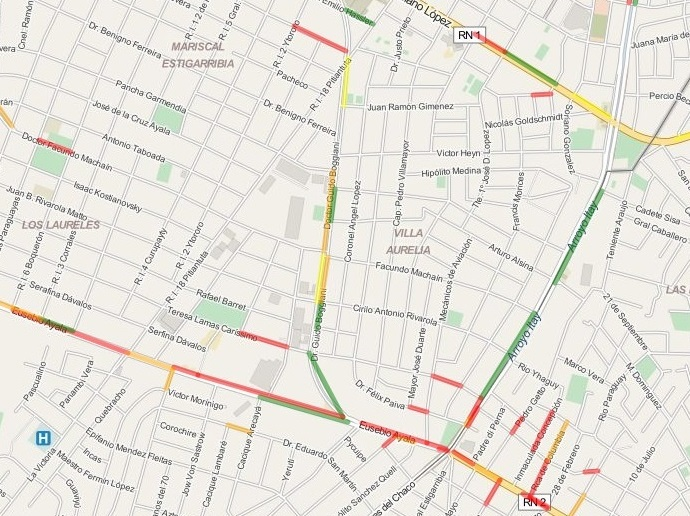
\includegraphics[width=0.45\textwidth]{apartados/figuras/estado_calles.jpg}
	\caption{\label{fig:calles} Estado de calles en Autotracks}	
\end{figure}
